\documentclass[11pt,compress,t,notes=noshow, xcolor=table]{beamer}
\usepackage[]{graphicx}\usepackage[]{color}
% maxwidth is the original width if it is less than linewidth
% otherwise use linewidth (to make sure the graphics do not exceed the margin)
\makeatletter
\def\maxwidth{ %
  \ifdim\Gin@nat@width>\linewidth
    \linewidth
  \else
    \Gin@nat@width
  \fi
}
\makeatother

\definecolor{fgcolor}{rgb}{0.345, 0.345, 0.345}
\newcommand{\hlnum}[1]{\textcolor[rgb]{0.686,0.059,0.569}{#1}}%
\newcommand{\hlstr}[1]{\textcolor[rgb]{0.192,0.494,0.8}{#1}}%
\newcommand{\hlcom}[1]{\textcolor[rgb]{0.678,0.584,0.686}{\textit{#1}}}%
\newcommand{\hlopt}[1]{\textcolor[rgb]{0,0,0}{#1}}%
\newcommand{\hlstd}[1]{\textcolor[rgb]{0.345,0.345,0.345}{#1}}%
\newcommand{\hlkwa}[1]{\textcolor[rgb]{0.161,0.373,0.58}{\textbf{#1}}}%
\newcommand{\hlkwb}[1]{\textcolor[rgb]{0.69,0.353,0.396}{#1}}%
\newcommand{\hlkwc}[1]{\textcolor[rgb]{0.333,0.667,0.333}{#1}}%
\newcommand{\hlkwd}[1]{\textcolor[rgb]{0.737,0.353,0.396}{\textbf{#1}}}%
\let\hlipl\hlkwb

\usepackage{framed}
\makeatletter
\newenvironment{kframe}{%
 \def\at@end@of@kframe{}%
 \ifinner\ifhmode%
  \def\at@end@of@kframe{\end{minipage}}%
  \begin{minipage}{\columnwidth}%
 \fi\fi%
 \def\FrameCommand##1{\hskip\@totalleftmargin \hskip-\fboxsep
 \colorbox{shadecolor}{##1}\hskip-\fboxsep
     % There is no \\@totalrightmargin, so:
     \hskip-\linewidth \hskip-\@totalleftmargin \hskip\columnwidth}%
 \MakeFramed {\advance\hsize-\width
   \@totalleftmargin\z@ \linewidth\hsize
   \@setminipage}}%
 {\par\unskip\endMakeFramed%
 \at@end@of@kframe}
\makeatother

\definecolor{shadecolor}{rgb}{.97, .97, .97}
\definecolor{messagecolor}{rgb}{0, 0, 0}
\definecolor{warningcolor}{rgb}{1, 0, 1}
\definecolor{errorcolor}{rgb}{1, 0, 0}
\newenvironment{knitrout}{}{} % an empty environment to be redefined in TeX

\usepackage{alltt}
\newcommand{\SweaveOpts}[1]{}  % do not interfere with LaTeX
\newcommand{\SweaveInput}[1]{} % because they are not real TeX commands
\newcommand{\Sexpr}[1]{}       % will only be parsed by R



\usepackage[english]{babel}
\usepackage[utf8]{inputenc}

\usepackage{dsfont}
\usepackage{verbatim}
\usepackage{amsmath}
\usepackage{amsfonts}
\usepackage{bm}
\usepackage{csquotes}
\usepackage{multirow}
\usepackage{longtable}
\usepackage{booktabs}
\usepackage{enumerate}
\usepackage[absolute,overlay]{textpos}
\usepackage{psfrag}
\usepackage{algorithm}
\usepackage{algpseudocode}
\usepackage{eqnarray}
\usepackage{arydshln}
\usepackage{tabularx}
\usepackage{placeins}
\usepackage{tikz}
\usepackage{setspace}
\usepackage{colortbl}
\usepackage{mathtools}
\usepackage{wrapfig}
\usepackage{bm}
\usetikzlibrary{shapes,arrows,automata,positioning,calc,chains,trees, shadows}
\tikzset{
  %Define standard arrow tip
  >=stealth',
  %Define style for boxes
  punkt/.style={
    rectangle,
    rounded corners,
    draw=black, very thick,
    text width=6.5em,
    minimum height=2em,
    text centered},
  % Define arrow style
  pil/.style={
    ->,
    thick,
    shorten <=2pt,
    shorten >=2pt,}
}
\usepackage{subfig}


% Defines macros and environments
\input{../../style/common.tex}
% \input{common.tex}

%\usetheme{lmu-lecture}
\newcommand{\titlefigure}{figure/eval_mclass_roc_sp_12_1}
\newcommand{\learninggoals}{
\item Understand the ROC curve
\item Be able to compute a ROC curve manually
\item Understand the definition of AUC and what a certain value of AUC means 
(and what not!)}
\usepackage{../../style/lmu-lecture}

\let\code=\texttt
\let\proglang=\textsf

\setkeys{Gin}{width=0.9\textwidth}

\title{Introduction to Machine Learning}
% \author{Bernd Bischl, Christoph Molnar, Daniel Schalk, Fabian Scheipl}
\institute{\href{https://compstat-lmu.github.io/lecture_i2ml/}{compstat-lmu.github.io/lecture\_i2ml}}
\date{}

\setbeamertemplate{frametitle}{\expandafter\uppercase\expandafter\insertframetitle}

\begin{document}

% This file loads R packages, configures knitr options and sets preamble.Rnw as parent file
% IF YOU MODIFY THIS, PLZ ALSO MODIFY setup.Rmd ACCORDINGLY...

% Defines macros and environments
\input{../../latex-math/basic-math.tex}
\input{../../latex-math/basic-ml.tex}
%! includes: evaluation-measures-classification-roc

\lecturechapter{Evaluation: Measures for Binary Classification: 
ROC Visualization}
\lecture{Introduction to Machine Learning}

% \begin{vbframe}{ROC Space}
% \end{itemize}
% \begin{center}
% \includegraphics[width=0.7\textwidth, height=5.0cm]{figure_man/roc-space1.png}
% \end{center}
% \end{vbframe}

% ------------------------------------------------------------------------------

\begin{vbframe}{Labels: ROC Space}

\begin{itemize}
 \item We characterize a classifier by its TPR and FPR values and plot them in 
 a coordinate system.
 \item We could also use two different ROC metrics which define a trade-off, 
 for instance, TPR and PPV.
\end{itemize}

\lz

\begin{minipage}[c]{0.5\textwidth}
  \begin{knitrout}
    \scriptsize
    \definecolor{shadecolor}{rgb}{0.969, 0.969, 0.969}\color{fgcolor}
    {\centering \includegraphics[width=\textwidth]{figure/eval_mclass_roc_sp_1}}
  \end{knitrout}
\end{minipage}%
\begin{minipage}[c]{0.5\textwidth}
% \includegraphics[width=\textwidth]{figure_man/roc-confmatrix2.png}
\begin{center}
  \small
  \begin{tabular}{cc|cc}
    & & \multicolumn{2}{c}{\bfseries True Class $y$} \\
    & & $+$ & $-$ \\
    \hline
    \bfseries Pred.     & $+$ & TP & FP \\
              $\yh$ & $-$ & FN & TN \\
\end{tabular}
\lz
$$\text{TPR} = \frac{\text{TP}}{\text{TP} + \text{FN}}$$
$$\text{FPR} = \frac{\text{FP}}{\text{FP} + \text{TN}}$$
\end{center}
\end{minipage}

\end{vbframe}

% ------------------------------------------------------------------------------

\begin{vbframe}{Labels: ROC Space}

\begin{itemize}
  \item The best classifier lies on the top-left corner, where FPR equals 0 and 
  TPR is maximal.
  \item The diagonal is worst as it corresponds to a classifier producing random 
  labels (with different proportions). 
\end{itemize}

\lz

\begin{minipage}[c]{0.5\textwidth}
  \begin{itemize}
    \item If each positive $x$ will be randomly classified 
    with 25\% as "pos", $\text{TPR} = 0.25$.
    \item If we assign each negative $x$ randomly to "pos", $\text{FPR} = 0.25$.
  \end{itemize}
\end{minipage}%
\begin{minipage}[c]{0.5\textwidth}
  \centering \includegraphics[width=0.8\textwidth]{figure/eval_mclass_roc_sp_2}
\end{minipage}

\end{vbframe}

% ------------------------------------------------------------------------------

\begin{vbframe}{Labels: ROC Space}

\begin{itemize}
  \item In practice, we should never obtain a classifier below the diagonal.
  \item Inverting the predicted labels ($0 \mapsto 1$ and $1 \mapsto 0$) will 
  result in a reflection at the diagonal. \\
  $\Rightarrow \text{TPR}_{\text{new}} = 1 - \text{TPR}$ and 
  $\text{FPR}_{\text{new}} = 1 - \text{FPR}.$ \\
\end{itemize}

\begin{center}
  \includegraphics[width=0.4\textwidth]{figure/eval_mclass_roc_sp_3}
\end{center}

\end{vbframe}

% ------------------------------------------------------------------------------

\begin{vbframe}{Label Distribution in TPR and FPR}

TPR and FPR (ROC curves) are insensitive to the class distribution in the sense 
that they are not affected by changes in the ratio $\np/\nn$ (at prediction).

\lz

\begin{columns}
  \begin{column}{0.45\textwidth}
  \underline{Example 1}:\\
  Proportion $\np/\nn = 1$\\
  \lz
  {
  \tiny
  \centering
  \tiny
  \begin{tabular}{|l|c|c|}
                  \hline
                 & Actual Positive & Actual Negative \\ \hline
  Pred. Positive & 40            & 25            \\ \hline
  Pred. Negative & 10            & 25           \\ \hline
  \end{tabular}
  }
  
  \medskip
  $\text{MCE} = 35/100 = 0.35$\\
  $\text{TPR} = 0.8$\\ 
  $\text{FPR} = 0.5$ 
\end{column}
\begin{column}{0.45\textwidth} 
  \underline{Example 2}:\\
  Proportion $\np/\nn = 2$\\
  \lz
  {
  \tiny
  \begin{tabular}{|l|c|c|}
                  \hline
                 & Actual Positive & Actual Negative \\ \hline
  Pred. Positive & 80            & 25            \\ \hline
  Pred. Negative & 20            & 25           \\ \hline
  \end{tabular}
  }
  
  \medskip
  $\text{MCE} = 45/150 = 0.3$\\
  $\text{TPR} = 0.8$\\ 
  $\text{FPR} = 0.5$ 
\end{column}
\end{columns}

\lz

Note: If class proportions differ during training, the above is not true. 
Estimated posterior probabilities can change!

\end{vbframe}

% ------------------------------------------------------------------------------

% \begin{vbframe}{Scoring Classifiers}
% \begin{itemize}
% \item A scoring classifier is a model which outputs scores or probabilities, instead of discrete labels, and nearly all modern classifiers can do that.
% \item Thresholding flexibly converts measured probabilities to labels.
%   Predict $1$ (positive class) if $\fxh > c$ else predict $0$.
% \item Normally we could use $c = 0.5$ to convert, but for imbalanced or cost-sensitive situations another threshold could be much better.
% \item After thresholding, any metric defined on labels can be used.
% \end{itemize}
% \begin{center}
% % FIGURE SOURCE: https://docs.google.com/presentation/d/1GmlgtjSCTHgSAveVGf-x1ojAjGP2llPhFKjn_6M4Sig/edit?usp=sharing
% \includegraphics[width=0.5\textwidth]{figure_man/confusion_matrix_measures}
% \end{center}
% \end{vbframe}

% ------------------------------------------------------------------------------

\begin{vbframe}{From Probabilities to Labels: ROC Curve}

Remember: Both probabilistic and scoring classifiers can output classes by 
thresholding:
$$\hx = [\pix) \ge c] \quad \text{ or } \quad \hx = [\fx \ge c].$$

% \begin{center}
%   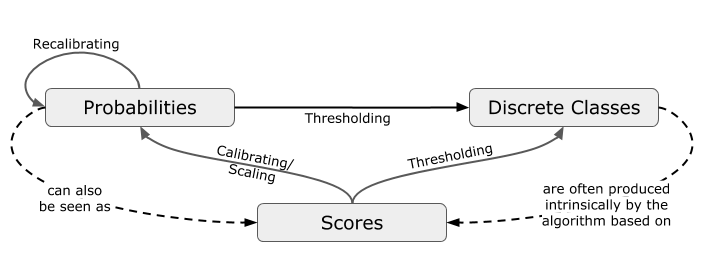
\includegraphics{../supervised-classification/figure_man/classifiers.png}
% \end{center}

\textbf{To draw a ROC curve}:

\lz

\begin{minipage}[b]{0.65\textwidth}
  \footnotesize
  \begin{enumerate}
    \item Rank test observations on decreasing score.
    \item Start with $c = 1$, so we start in $(0, 0)$; we predict everything as
    negative.
    \item Iterate through all possible thresholds $c$ and proceed for each
    observation $x$ as follows:
    \begin{itemize}
      \footnotesize
      \item If $x$ is positive, move TPR $1/n_+$ up, \\as we have one TP more.
      \item If $x$ is negative, move FPR $1/n_-$ right, \\as we have one FP 
      more.
    \end{itemize}
  \end{enumerate}
\end{minipage}%
\begin{minipage}[b]{0.35\textwidth}
  \centering
  \includegraphics[width=\textwidth]{figure/eval_mclass_roc_sp_4}
\end{minipage}

\end{vbframe}

% ------------------------------------------------------------------------------

\begin{vbframe}{Drawing ROC Curves}

% new frame for every animation step (rather than framebreak) to prevent plots
% from jumping

\begin{knitrout}\scriptsize
\definecolor{shadecolor}{rgb}{0.969, 0.969, 0.969}\color{fgcolor}

{
% \centering 
\includegraphics[width=0.8\textwidth]{figure/eval_mclass_roc_sp_5} 
}

\end{knitrout}

\vfill

\begin{minipage}[b]{0.3\textwidth}
  $c =$ 0.9\\ 
  $\rightarrow$ TPR = 0.167 \\
  $\rightarrow$ FPR = 0
\end{minipage}%
\begin{minipage}[b]{0.7\textwidth}
  \textcolor{blue}{add plot showing sliding thresholds (suggestion Ludwig)}
\end{minipage}

\end{vbframe}

% ------------------------------------------------------------------------------

\begin{vbframe}{Drawing ROC Curves}

\begin{knitrout}\scriptsize
\definecolor{shadecolor}{rgb}{0.969, 0.969, 0.969}\color{fgcolor}

{
% \centering 
\includegraphics[width=0.8\textwidth]{figure/eval_mclass_roc_sp_6}
}

\end{knitrout}

\vfill

\begin{minipage}[b]{0.3\textwidth}
  $c =$ 0.85\\ 
  $\rightarrow$ TPR = 0.333 \\
  $\rightarrow$ FPR = 0
\end{minipage}%
\begin{minipage}[b]{0.7\textwidth}
  \textcolor{blue}{add plot showing sliding thresholds (suggestion Ludwig)}
\end{minipage}

\end{vbframe}

% ------------------------------------------------------------------------------

\begin{vbframe}{Drawing ROC Curves}

\begin{knitrout}\scriptsize
\definecolor{shadecolor}{rgb}{0.969, 0.969, 0.969}\color{fgcolor}

{
% \centering 
\includegraphics[width=0.8\textwidth]{figure/eval_mclass_roc_sp_7}
}

\end{knitrout}

\vfill

\begin{minipage}[b]{0.3\textwidth}
  $c =$ 0.66\\ 
  $\rightarrow$ TPR = 0.5 \\
  $\rightarrow$ FPR = 0
\end{minipage}%
\begin{minipage}[b]{0.7\textwidth}
  \textcolor{blue}{add plot showing sliding thresholds (suggestion Ludwig)}
\end{minipage}

\end{vbframe}

% ------------------------------------------------------------------------------

\begin{vbframe}{Drawing ROC Curves}

\begin{knitrout}\scriptsize
\definecolor{shadecolor}{rgb}{0.969, 0.969, 0.969}\color{fgcolor}

{
% \centering 
\includegraphics[width=0.8\textwidth]{figure/eval_mclass_roc_sp_8}
}

\end{knitrout}

\vfill

\begin{minipage}[b]{0.3\textwidth}
  $c =$ 0.6\\ 
  $\rightarrow$ TPR = 0.5 \\
  $\rightarrow$ FPR = 0.167
\end{minipage}%
\begin{minipage}[b]{0.7\textwidth}
  \textcolor{blue}{add plot showing sliding thresholds (suggestion Ludwig)}
\end{minipage}

\end{vbframe}

% ------------------------------------------------------------------------------

\begin{vbframe}{Drawing ROC Curves}

\begin{knitrout}\scriptsize
\definecolor{shadecolor}{rgb}{0.969, 0.969, 0.969}\color{fgcolor}

{
% \centering 
\includegraphics[width=0.8\textwidth]{figure/eval_mclass_roc_sp_9}
}

\end{knitrout}

\vfill

\begin{minipage}[b]{0.3\textwidth}
  $c =$ 0.55\\ 
  $\rightarrow$ TPR = 0.667 \\
  $\rightarrow$ FPR = 0.167
\end{minipage}%
\begin{minipage}[b]{0.7\textwidth}
  \textcolor{blue}{add plot showing sliding thresholds (suggestion Ludwig)}
\end{minipage}

\end{vbframe}

% ------------------------------------------------------------------------------

\begin{vbframe}{Drawing ROC Curves}

\begin{knitrout}\scriptsize
\definecolor{shadecolor}{rgb}{0.969, 0.969, 0.969}\color{fgcolor}

{
% \centering 
\includegraphics[width=0.8\textwidth]{figure/eval_mclass_roc_sp_10} 
}

\end{knitrout}

\vfill

\begin{minipage}[b]{0.3\textwidth}
  $c =$ 0.3\\ 
  $\rightarrow$ TPR = 0.833 \\
  $\rightarrow$ FPR = 0.5
\end{minipage}%
\begin{minipage}[b]{0.7\textwidth}
  \textcolor{blue}{add plot showing sliding thresholds (suggestion Ludwig)}
\end{minipage}

\end{vbframe}

% ------------------------------------------------------------------------------

\begin{vbframe}{Drawing ROC Curves}

\begin{knitrout}\scriptsize
\definecolor{shadecolor}{rgb}{0.969, 0.969, 0.969}\color{fgcolor}

{
% \centering 
\includegraphics[width=0.8\textwidth]{figure/eval_mclass_roc_sp_11}
}

\end{knitrout}

\end{vbframe}

% ------------------------------------------------------------------------------

\begin{vbframe}{ROC Curve properties}

\begin{minipage}[c]{0.5\textwidth}
  \begin{itemize}
    \item The closer the curve to the top-left corner, the better.
    \item If ROC curves cross, a different model might be better in different 
    parts of the ROC space.
\end{itemize}
\end{minipage}%
\begin{minipage}[c]{0.5\textwidth}
  \centering 
  \includegraphics[width=\textwidth]{figure/eval_mclass_roc_sp_12}
\end{minipage}

\lz

\begin{itemize}
  \item Small thresholds will very liberally predict the positive class, and 
  result in a potentially higher FPR, but also higher TPR.
  \item High thresholds will very conservatively predict the positive class, 
  and result in a lower FPR and TPR.
  \item As we have not defined the trade-off between false postives and false 
  negative costs, we cannot easily select the "best" threshold. \\
  $\rightarrow$ Visual inspection of all possible results seems useful.
\end{itemize}

% \textcolor{blue}{Include figure?}
% 
% \begin{center}
%   \includegraphics[width=\textwidth]{figure_man/roc-curves2.png}
% \end{center}

% \textcolor{blue}{Include this again or compare it with above?}
%  \begin{itemize}
%    \item Rank test observations on decreasing score
%    \item Set $\alpha=1$, so we start in $(0, 0)$; we predict everything as "neg"
%    \item For each observation $x$ (in the decreasing order).
%    \begin{itemize}
%      \item Reduce threshold, so prediction for next observation changes
%      \item If $x$ is "pos", move TPR $1/n_+$ up, as we have one TP more
%      \item If $x$ is "neg", move FPR $1/n_-$ right, as we have one FP more
%    \end{itemize}
%  \end{itemize}

\end{vbframe}

% ------------------------------------------------------------------------------

% \begin{vbframe}{ROC Curve}
% \begin{itemize}
%   \item The closer the curve to the top-left corner, the better
%   \item If ROC curves cross, a different model can be better in different parts 
%   of the ROC space
% \end{itemize}
% \begin{knitrout}\scriptsize
% \definecolor{shadecolor}{rgb}{0.969, 0.969, 0.969}\color{fgcolor}
% 
% {\centering \includegraphics[width=.65\textwidth]{figure/eval_mclass_roc_sp_12} 
% 
% }
% 
% \end{knitrout}
% \end{vbframe}

% ------------------------------------------------------------------------------

\begin{vbframe}{AUC: Area Under ROC Curve}

\begin{itemize}
  % \small
  \item AUC $\in [0,1]$ is a single metric to evaluate scoring classifiers --
  independent of the chosen threshold.
  \begin{itemize}
    \item AUC = 1: perfect classifier
    \item AUC = 0.5: random, non-discriminant classifier
    \item AUC = 0: perfect, with inverted labels
  \end{itemize}
  \item The AUC is directly related to the Gini coefficient $G$: 
  $\text{AUC} = 0.5 \cdot (G + 1)$. 
  \textcolor{blue}{@BB: check if correct/helpful here}
\end{itemize}

\begin{center}
  \includegraphics[width=0.5\textwidth]{figure/eval_mclass_roc_sp_12_1}
\end{center}

\end{vbframe}

% ------------------------------------------------------------------------------

% 
% \begin{vbframe}{AUC: Area Under ROC Curve}
% Interpretation: Probability that classifier ranks a random positive higher than a random negative observation
% 
% \begin{center}
% % FIGURE SOURCE: https://docs.google.com/presentation/d/1xj9_84181bqFpr0EMqdGHE6dUf_vAf1qcs9z-siUsCw/edit?usp=sharing
% \includegraphics[width=0.8\textwidth,page=1]{figure_man/auc_interpretation.pdf}
% \end{center}
% 
% \end{vbframe}


% \begin{vbframe}{Partial AUC}
% \begin{itemize}
%   \item Sometimes it can be useful to look at a \href{http://journals.sagepub.com/doi/pdf/10.1177/0272989X8900900307}{specific region under the ROC curve}  $\Rightarrow$ partial AUC (pAUC).
%   \item Examples: focus on a region with low FPR or a region with high TPR:
% \end{itemize}
% 
% \begin{knitrout}\scriptsize
% \definecolor{shadecolor}{rgb}{0.969, 0.969, 0.969}\color{fgcolor}
% 
% {\centering \includegraphics[width=0.9\textwidth]{figure/eval_mclass_roc_sp_13} 
% 
% }

% \end{knitrout}

% ------------------------------------------------------------------------------

\endlecture
\end{document}
